% =====================================================================
% APÊNDICE A: tabelas e figura de detalhe (movidas da seção 4 em 4/11/2026
% para caber no limite de 20 páginas; o conteúdo não mudou).
% =====================================================================
\clearpage
\section*{APÊNDICE A -- RESULTADOS DETALHADOS}
\addcontentsline{toc}{section}{APÊNDICE A -- RESULTADOS DETALHADOS}

\begin{table}[H]
\centering
\flutuante{%
% gerado por gerar_tabelas_extras.py; nao editar a mao
{\footnotesize\setlength{\tabcolsep}{3pt}
\begin{tabular}{llrrrrr}
\toprule
Consulta & Classe & Original & Só reescrita & Só índice & Prescrição & Nativo \\
\midrule
F1 & AP1 & 800.856 & 800.856 & 8.330 & 47 & -- \\
F2 & AP1 & 7.405 & 7.405 & 1.282 & 3 & -- \\
F3 & AP1 & 46.704 & 46.704 & 27.638 & 50 & -- \\
F4 & AP1 & 800.856 & 800.856 & 8.330 & 4.839 & -- \\
F5$^{*}$ & AP1 & 46.704 & 46.704 & 50 & 50 & -- \\
S1 & AP2 & 2.409.973 & 808.261 & 57.988 & 24.239 & -- \\
S2 & AP2 & 894.264 & 847.560 & 873.692 & 837.274 & 93.431 \\
S3 & AP2 & 1.138.570 & 969.713 & 818.160 & 809.506 & 337.737 \\
S4 & AP2 & 808.261 & 808.261 & 13.875 & 22.636 & -- \\
S5$^{*}$ & AP2 & 13.952 & 13.952 & 9.319 & 9.319 & 6.570 \\
C1 & AP3 & 800.856 & 800.856 & 46.157 & 41 & 2.845 \\
C2 & AP3 & 800.856 & 800.856 & 227 & 3 & 14 \\
C3 & AP3 & 168.857 & 168.857 & 54.311 & 40 & 615 \\
C4 & AP3 & 7.405 & 7.405 & 7.405 & 32 & 164 \\
V1 & AP4 & 46.704 & -- & -- & 3 & -- \\
V2 & AP4 & 168.857 & -- & -- & 27 & -- \\
V3 & AP4 & 6.547 & -- & -- & 9 & -- \\
V4 & AP4 & 800.856 & -- & -- & 11 & -- \\
V5 & AP4 & 7.405 & -- & -- & 82 & -- \\
\bottomrule
\end{tabular}\par
\vspace{3pt}
\begin{minipage}{\linewidth}\footnotesize
Mediana das leituras lógicas, cenário quente. Prescrição = reescrita com índice (classes 1 a 3) ou só o índice (classe 4). \texttt{--}: braço inexistente ou sem sugestão distinta do índice do \textit{framework}. $^{*}$ Consulta de controle.
\end{minipage}}
%
}{\caption{Leituras lógicas medianas por consulta e braço, cenário quente}
\label{tab:bracos}}{Fonte: Do autor.}
\end{table}

\begin{figure}[H]
\centering
\flutuante{%
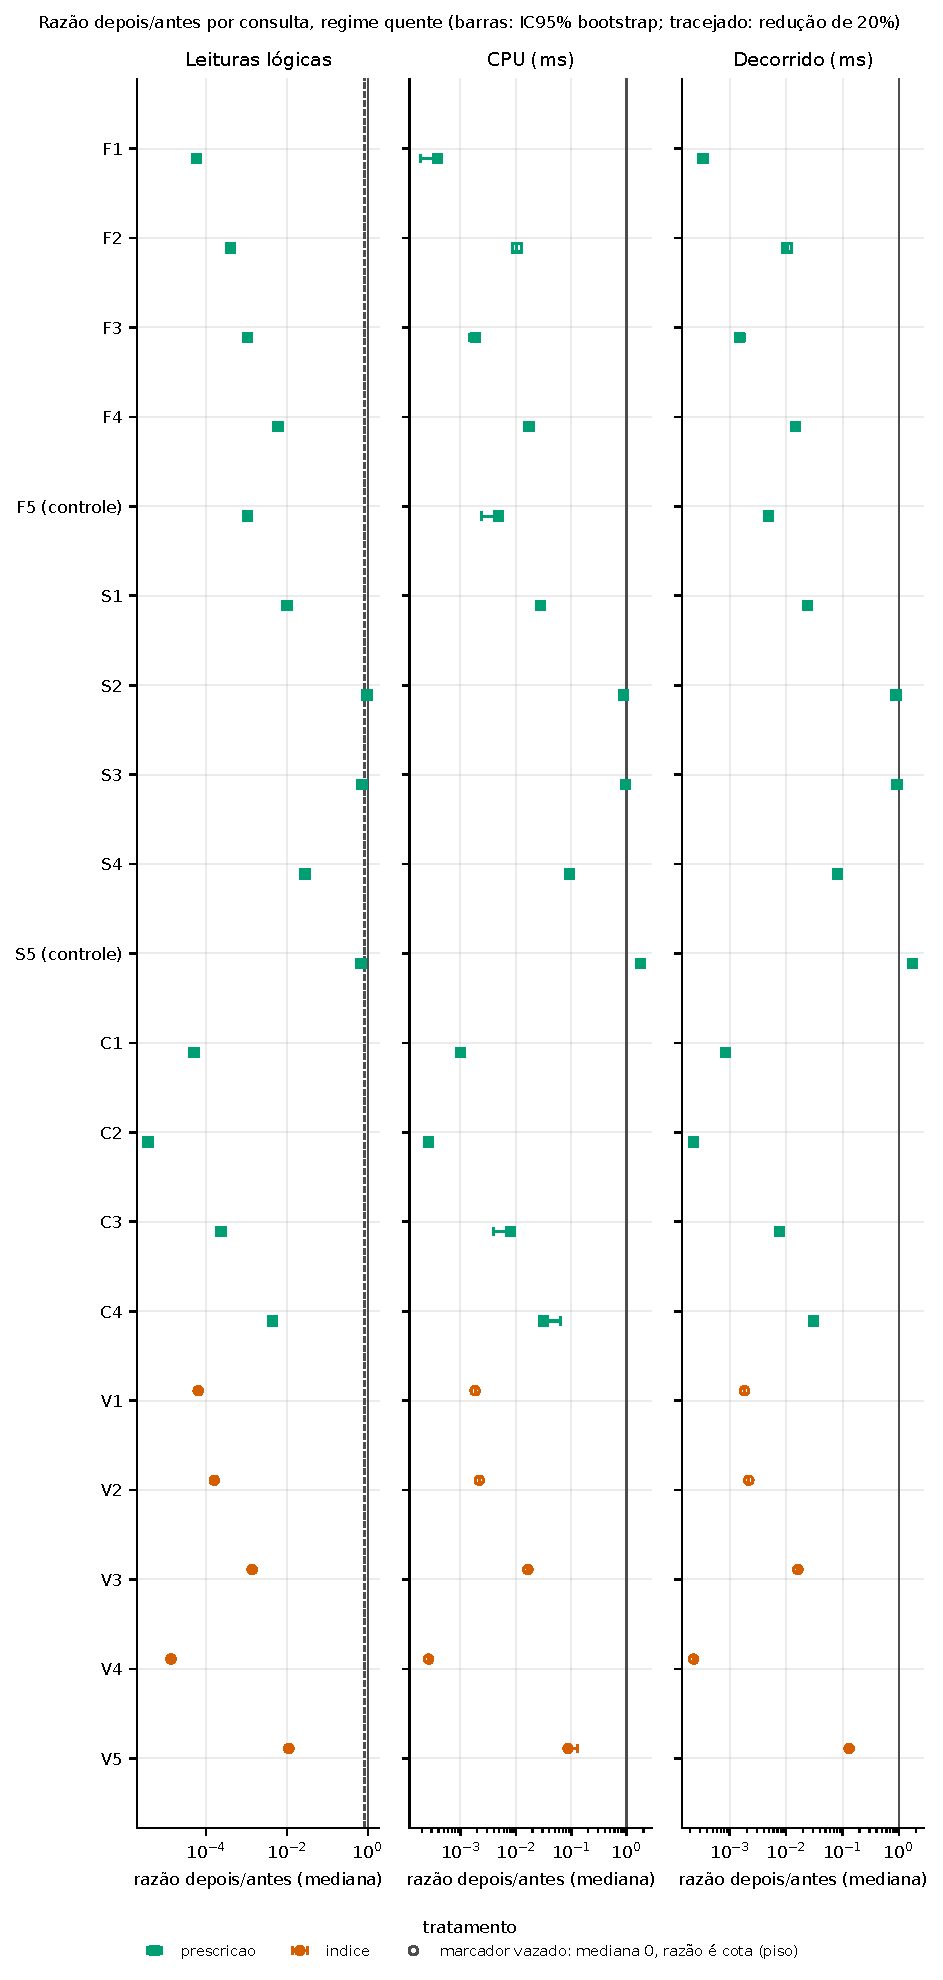
\includegraphics[width=\textwidth,height=0.78\textheight,keepaspectratio]{dados/r2/figuras/razao_por_consulta_quente.pdf}%
}{\caption{Razão entre as medições depois e antes, por consulta e métrica, cenário quente}
\label{fig:razao}}{Fonte: Do autor.}
\end{figure}

\begin{table}[H]
\centering
\flutuante{%
% gerado por gerar_tabelas_extras.py a partir de escrita-corrigida; nao editar a mao
{\footnotesize\setlength{\tabcolsep}{2.5pt}
\begin{tabular}{lrrrrrrr}
\toprule
 &  & \multicolumn{3}{c}{Leituras lógicas} & \multicolumn{3}{c}{Bytes de log} \\
\cmidrule(lr){3-5}\cmidrule(lr){6-8}
Índice & Págs. & \texttt{INS} & \texttt{UPD} & \texttt{DEL} & \texttt{INS} & \texttt{UPD} & \texttt{DEL} \\
\midrule
Badges(UserId) & 1.914 & 2,12 & 668 & 334 & 4,59 & 2,83 & 1,77 \\
Comments(PostId) +Score & 8.652 & 1,47 & 145 & 70,8 & 1,26 & 2,90 & 1,27 \\
Comments(UserId) & 6.724 & 1,18 & 137 & 69,2 & 1,86 & 2,83 & 1,26 \\
Comments(UserId) +PostId, Score & 10.560 & 1,47 & 137 & 69,2 & 1,26 & 2,96 & 1,28 \\
Comments(UserId) +4 colunas$^{\dagger}$ & 167.145 & 1,68 & 183 & 91,9 & 1,90 & 7,79 & 1,99 \\
Posts(CreationDate) & 8.330 & 1,41 & 31,6 & 15,8 & 1,06 & 2,90 & 1,07 \\
Posts(OwnerUserId) & 6.470 & 1,32 & 31,2 & 15,8 & 1,68 & 2,83 & 1,07 \\
Posts(OwnerUserId) +Score, CreationDate & 12.023 & 1,41 & 31,2 & 15,8 & 1,07 & 3,03 & 1,08 \\
Posts(OwnerUserId) +Score, ViewCount & 10.162 & 1,42 & 31,1 & 15,8 & 1,06 & 2,96 & 1,07 \\
Posts(OwnerUserId, Score) & 8.333 & 1,41 & 31,2 & 15,8 & 1,06 & 2,90 & 1,07 \\
Posts(Score, OwnerUserId) & 8.333 & 1,41 & 31,1 & 15,8 & 1,06 & 2,90 & 1,07 \\
Posts(OwnerUserId) +18 colunas$^{\dagger}$ & 863.949 & 1,76 & 41,9 & 20,5 & 1,95 & 27,7 & 1,99 \\
Users(DisplayName) +Reputation & 1.282 & 2,62 & 89,9 & 44,3 & 13,6 & 2,82 & 1,25 \\
Users(Location) & 847 & 1,29 & 85,5 & 43,3 & 1,86 & 2,98 & 1,26 \\
Users(Location) +DisplayName, Reputation & 1.772 & 2,68 & 85,5 & 43,3 & 14,1 & 3,33 & 1,30 \\
Users(Reputation) +DisplayName & 1.279 & 2,62 & 85,5 & 43,3 & 13,9 & 3,22 & 1,25 \\
Users(Location) +12 colunas$^{\dagger}$ & 7.354 & 2,60 & 85,5 & 43,3 & 18,3 & 8,56 & 2,00 \\
Votes(CreationDate) +VoteTypeId & 27.638 & 1,80 & 798 & 384 & 1,86 & 2,96 & 1,88 \\
Votes(PostId) & 17.589 & 1,61 & 798 & 384 & 1,80 & 2,83 & 1,82 \\
Votes(PostId) +CreationDate & 27.624 & 1,61 & 798 & 384 & 1,86 & 2,96 & 1,88 \\
\bottomrule
\end{tabular}\par
\vspace{3pt}
\begin{minipage}{\linewidth}\footnotesize
Razão com/sem o índice, mediana de 10 repetições de 1.000 linhas por operação (\texttt{INS} = \texttt{INSERT}, \texttt{UPD} = \texttt{UPDATE} da coluna-chave, \texttt{DEL} = \texttt{DELETE}), dentro de transação desfeita, nas mesmas linhas com e sem o índice. $^{\dagger}$ Índice sugerido pelo recurso nativo. Sem limiar de aceitação: o custo é reportado, não julgado.
\end{minipage}}
%
}{\caption{Custo de escrita por índice (razão com/sem o índice)}
\label{tab:escrita}}{Fonte: Do autor.}
\end{table}
